\chapter{Application Layer}
\label{chapter:applicationlayer}

% OVERVIEW
\section{Overview}
This section gives an overview over the components of the applacation layer (GUI) of ACE. Figure \ref{applicationlayer_ace_overview} shows the graphical user interface (GUI) with all components. Each component is explained detailed in section \ref{applicationlayer_components}.
\begin{figure}[H]
\begin{center}
  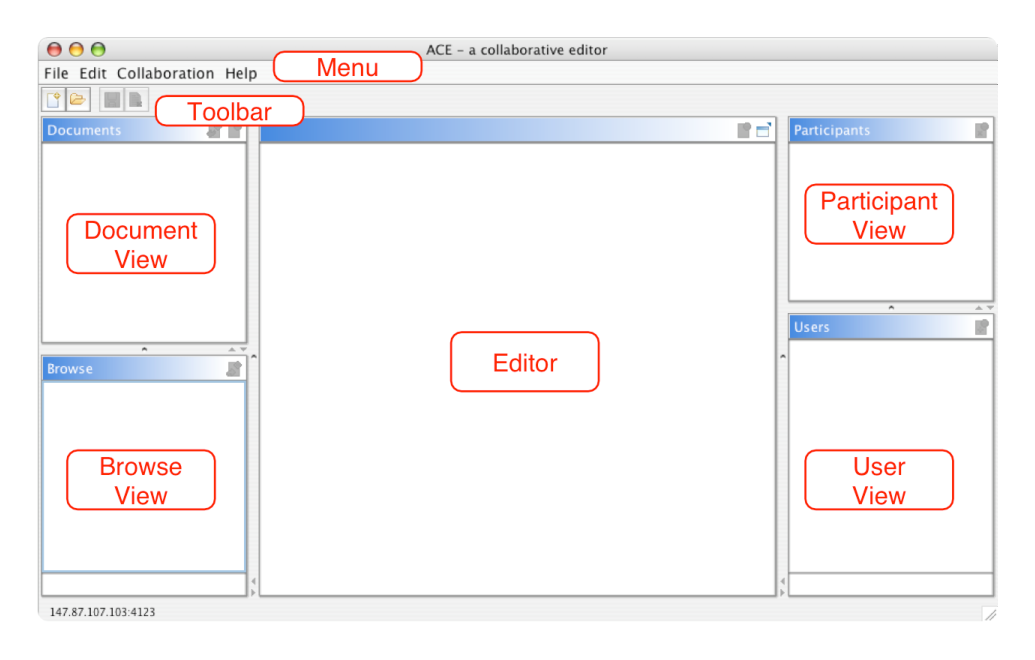
\includegraphics[height=3.135in, width=5.01in]{../images/finalreport/application_ace_overview.eps}
\caption{ACE Overview}
\label{applicationlayer_ace_overview}
\end{center}
\end{figure}
On the top of the application are the menubar and the toolbar. The menubar is splitted into four menus which are containing functions associated to their category. Below the menubar is the toolbar that contains the most used functions out of the menu.

In the middle of the GUI are the four views and the editor component. The document view shows the current opened documents, the browse view contains all documents that can be found over the network (published by other users), the user view shows all users running ACE in the same network and the participant view contains a list of all users that are currently editing in the selected document.

At the bottom of the application is the status bar that simple contains a label which dispays the current IP address.

% COMPONENTS
\section{Components}
\label{applicationlayer_components}
% FRAME
\subsection{Frame}


% MENU
\subsection{Menu}

% TOOLBAR
\subsection{Toolbar}

% VIEWS
\subsection{Views \& View Controllers}
\subsubsection{Overview}
\subsubsection{Document View}
\subsubsection{Browse View}
\subsubsection{User View}
\subsubsection{Participant View}

% ACTIONS
\subsection{Actions}

% EDITOR
\subsection{Editor}
This section gives an overview of all components needed for the collaborative editor. The following figure shows the class diagram:
\begin{figure}[H]
\begin{center} \frame{
  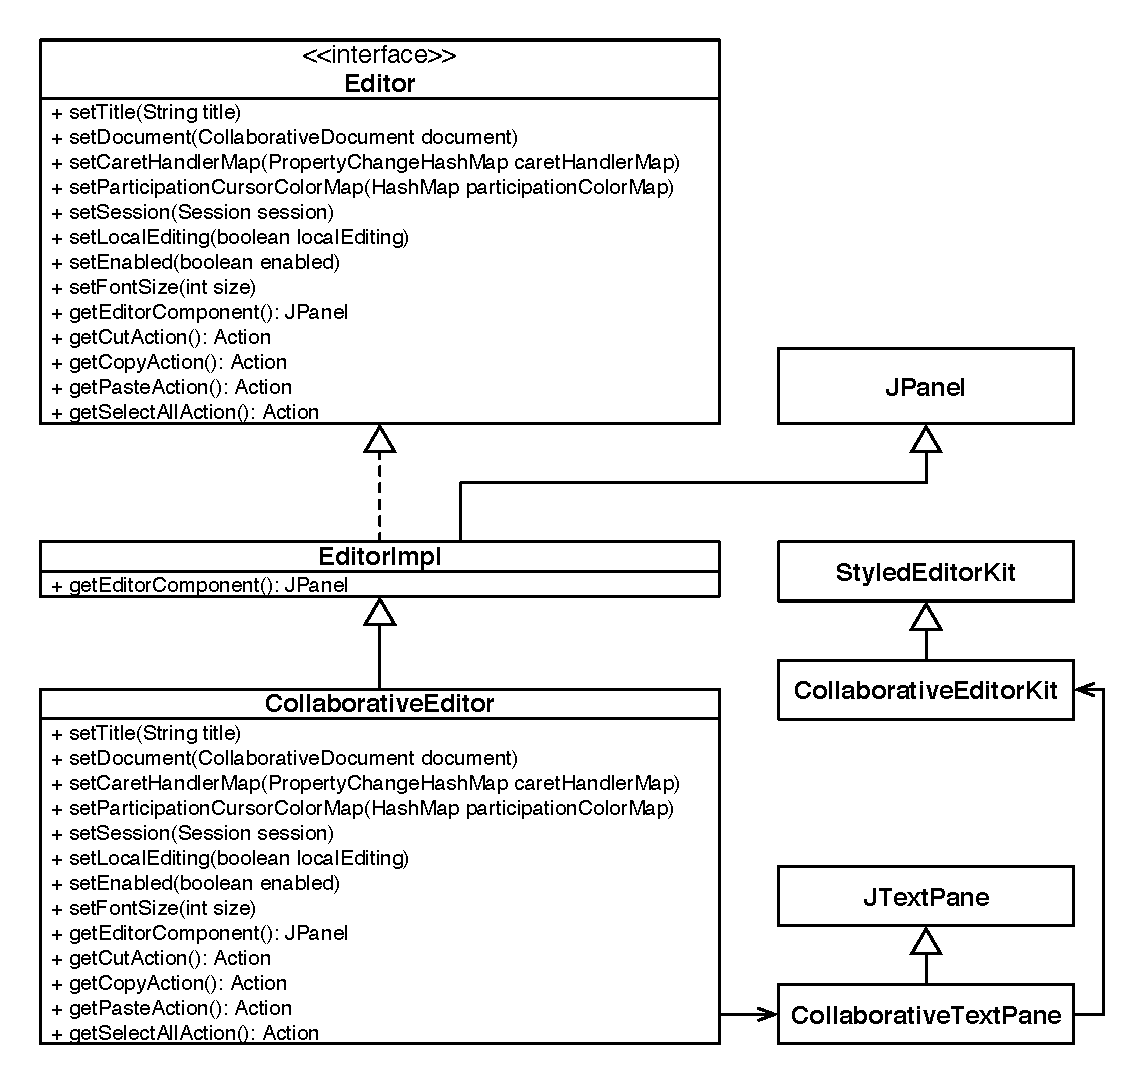
\includegraphics[height=5.25in, width=5.55in]{../images/finalreport/application_editor.eps}
  }
\caption{Collaborative Editor Class Diagram}
\label{default}
\end{center}
\end{figure}

\subsubsection{Collaborative Editor}
The collaborative editor is a JFrame which support all functionality defined in the \textit{Editor} interface. The constructor looks like:
\begin{verbatim}
  public CollaborativeEditor(...) {
    // create editor pane & kit
    cTextPane = new CollaborativeTextPane();
    cEditorKit = new CollaborativeEditorKit();
    cTextPane.setEditorKit(cEditorKit);

    // create editor pane
    JScrollPane scrollPane = new JScrollPane(cTextPane);
    editorPane = new SimpleInternalFrame(null, " ", editorToolBar, scrollPane);

    // add components		
    setLayout(new BorderLayout());
    add(editorPane);    
  }
\end{verbatim}

All setter methods (except \texttt{setTitle(...)} that sets directly the tilte of the frame) are directly forwarded to the collaborative text pane (\texttt{cTextPane}) like:
\begin{verbatim}
  public void setXYZ(...) {
    cTextPane.setXYZ(...);
  }
\end{verbatim}

To use the standard text component actions for the menu \textit{edit}, we need getter methods that returns them. All text component actions are handled in the editor kit (see section \ref{collaborative_editor_kit}), thus we forward the getter methods to the collaborative editor kit (\texttt{cEditorKit}):
\begin{verbatim}
  public Action getXYZAction() {
    return cEditorKit.getXYZAction();
  }
\end{verbatim}



\subsubsection{Collaborative TextPane}
The collaboration text pane implements all functionality defined by the \texttt{Editor} interface. This component overrides the \texttt{replaceSelection} method from its superclass \texttt{JTextPane}. This is needed to use a lock while inserting content into the document. Locking has to be done to avoid asynchronous text insertions while creating and sending operations that are based on the document content.
\begin{verbatim}
  public void replaceSelection(String content) {
    SessionTemplate template = new SessionTemplate(session);
    template.execute(new SessionTemplateCallback() {
      public void execute(Session session) {

        // create and send operation
        Operation op  = new Delete/InsertOperation(...);
        session.sendOperation(op);

        // call superclass method
        CollaborativeTextPane.super.replaceSelection(content);
      }
    }
  }
\end{verbatim}
Furthermore there is a method \texttt{setCaretHandlerMap(PropertyChangeHashMap caretHandlerMap)} which is responsible to set the map with the carets (cursor positions) from all participants of the current document. The \texttt{PropertyChangeHashMap} is a map that adds a \texttt{PropertyChangeListener} on all inserted elements (carets from other users) and forwards their \texttt{PropertyChangeEvents} to all registered components. The following code fragment makes the editor able to receive updates if the carets of other users have changed:
\begin{verbatim}
  public void setCaretHandlerMap(PropertyChangeHashMap caretHandlerMap) {
    // unregister old map
    this.caretHandlerMap.removePropertyChangeListener(this);
    this.caretHandlerMap = caretHandlerMap;

    // register new map
    this.caretHandlerMap.addPropertyChangeListener(this);
  }
\end{verbatim}
To handle the own caret changes its necessary to register a \texttt{CaretListener}. The invoked method \texttt{caretUpdate(...)} checks if the current user really changed his cursor position and needs to send the new caret position to the session.

Each time a caret of another user changes the method \texttt{propertyChange(PropertyChangeEvent evt)} will be invoked. The \texttt{PropertyChangeEvent} contains the old and the new caret position from the users that moved his caret and forces a repaint. The implementation looks like:
\begin{verbatim}
  public void propertyChange(PropertyChangeEvent evt) {
    // old caret
    CaretUpdate oldCU = (CaretUpdate)evt.getOldValue();
    Rectangle oldRect = modelToView(oldCU.getDot());
    repaint(oldRect);

    // new caret
    CaretUpdate newCU = (CaretUpdate)evt.getNewValue();
    Rectangle newRect = modelToView(newCU.getDot());
    repaint(newRect);
  }
\end{verbatim}
The \texttt{repaint(...)} is eighter called by swing or explicit by the \texttt{propertyChange} method when one of the participant changed his cursor position. It iterates through the \texttt{caretHandlerMap} and paints the caret for each map entry.

\subsubsection{Collaborative EditoKit}
\label{collaborative_editor_kit}
The collaborative editor kit extends the styled editor kit and is needed for synchronisation purposes. To ensure the correct content of the text component its necessary to use lockings before sending operation for the following situations:
\begin{itemize}
\item \texttt{DeletePrevCharAction} which is called when the users presses the backspace key.
\item \texttt{DeleteNextCharAction} which is called when the users presses the delete key.
\item \texttt{CutAction} which is called when the user cuts some text out of the document.
\item Inserting Content: this issue is handled in the \textit{collaborative text pane}.
\end{itemize}

All editor actions are defined in an array that can be get by using the \texttt{getActions()} method from the superclass. The three delete actions listed above need to replaced by actions that are able to use locks. A simple solution would be:
\begin{verbatim}
  public class CollaborativeDeletePrevCharAction extends
    DefaultEditorKit.DeletePrevCharAction {
    
    public void actionPerformed(...) {
      // lock here
      super.actionPerformed(...);
      
      session.sendOperation(...)
      // unlock here
    }
  }
\end{verbatim}
Unfortunately its not possible to subclass the actions defined in the \texttt{DefaultEditorKit}. This leads to the solution to copy their implementation into the \texttt{CollaborativeEditorKit} and manipulate them. For example the \texttt{actionPerformed} method from \texttt{DeletePrevCharAction} looks like:
\begin{verbatim}
  public void actionPerformed(...) {
    SessionTemplate template = new SessionTemplate(session);
    template.execute(new SessionTemplateCallback() {
      public void execute(Session session) {

        // check whatever needed here and manipulate text component document
        document.remove(...);
        
        // create and send operation
        Operation op  = new DeleteOperation(...);
        session.sendOperation(op);

      }
    }
  }
\end{verbatim}


\subsubsection{Editor Controller}
The editor controller is registered for item selection change events from the \textit{DocumentViewController} and is used to enabled, disable and set editor values. Each time the selection is changed or the current document item changes properties, the following procedure is made:
\begin{itemize}
\item \textit{disable} the editor if no document is selected.
\item \textit{set} the \textit{document} of the selected item.
\item \textit{set} the editor \textit{title}.
\end{itemize}
Furthermore if the selected document is a published or a joined (remote) document the \textit{session} and the \textit{participant list} are set too.

\subsubsection{Collaborative Document}
The collaborative document extends the \textit{DefaultStyledDocument}. It is used for getting write locks and applying text styles. Each time a style added to the document changes the method \texttt{reapplyStyles(...)} is called.
\begin{verbatim}
  protected void styleChanged(Style style) {
    if(!style.getName().equals("default")) {
      reapplyStyles(style);
    }
  }
\end{verbatim}

The method \texttt{reapplyStyles(...)} iterates through all the text elements from the document and checks if they are using the changed style. All elements using this style will be notified and updated. The following scenario will work now and all text elements will have the new background color:
\begin{verbatim}
  // add style
  Style myStyle = document.addStyle("myStyle", null);
  StyleConstants.setBackground(myStyle, Color.BLUE);
  
  // insert some text here
  doc.insertString(...);
  
  // change style
  StyleConstants.setBackground(myStyle, Color.RED);
\end{verbatim}

\subsubsection{AsyncCaret}
When inserting text into a text component and setting the caret position asynchronous, its possible that the caret isnt set to the correct position. Asynchronous caret update is implemented in Java 1.4 but there is no posibility to enable it (this problem is solved in Java 1.5). \texttt{AsyncCaret} is a simple copy of the standard caret class with the following constructor details:
\begin{verbatim}
  public AsyncCaret() {
    async = true;
  }
\end{verbatim}

% OTHER
\subsection{Other}
\subsubsection{Application Controller}
\subsubsection{Application Factory}
\subsubsection{Dialog Controller}
\subsubsection{Persistent Content Pane}



\newpage
% WORKFLOWS
\section{Workflows}

% STARTUP
\subsection{Startup}
All the startup processes for ACE are defined in the main method from the class \textit{Main.java}:
\begin{description}
\item[1. Load Customizer ] The first step is to get the customizers. Customizers are used to create operating system based stuff like setting the look \& feel of the application.
\item[2. Load ApplicationContext ] After the customizer has been loaded, the spring application context (see \ref{} for more details about spring) needs to be loaded.
\item[3. Get ApplicationFactory ] The application factory is used to create all GUI components.
\item[4. Get ApplicationController ]  
\item[5. Get CollaborationService ] 
\item[6. Load PreferencesStore ]
\item[7. Create Main Frame ]
\item[8. Init PreferencesStore ]
\item[9. Init CollaborationService ]
\item[10. Create Empty Document ]
\end{description}




% ACTION ENABLING
\subsection{Enabling of Actions}


